\documentclass{rapport}
\usepackage{lipsum}
\usepackage{tikz}
\usepackage{wrapfig}
\title{Rapport UCL - Template} %Titre du fichier

\begin{document}

%----------- Informations du rapport ---------

\unif{EURECOM}
\titre{S5 PROJECT REPORT} %Titre du fichier .pdf
% \cours{Nom du cours} %Nom du cours
% \sujet{Sujet du rapport} %Nom du sujet


%----------- Initialisation -------------------
        
\fairemarges %Afficher les marges
\fairepagedegarde %Créer la page de garde
\tableofcontents%Créer la table de matières
\newpage

%------------ Corps du rapport ----------------

\section{Technical manual}

\subsection{Image processing part}

The first step toward computing the image and giving an angle is the image acquisition. We use the python library \verb|picamera| in order to get the camera's images, at a quite low quality, because it has proven to be more time-efficient.

% Gui tu peux changer le wrapfigure par des colonnes ou tout ce que tu veux
\begin{wrapfigure}{r}{.2\textwidth}
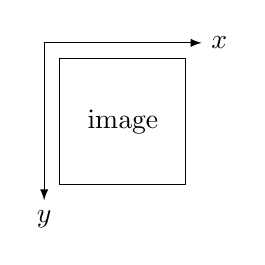
\begin{tikzpicture}[scale=2]
\draw[-latex] (0,0) -- (1,0);
\draw[-latex] (0,0) -- (0,-1);
\draw (0.1,-0.1) rectangle (0.9, -0.9);
\draw (0.5,-0.5) node {image};
\draw (1,0) node[right] {\(x\)};
\draw (0,-1) node[below] {\(y\)};
\end{tikzpicture}
\end{wrapfigure}

The frames are then read by openCV and converted into grey. OpenCV represents images with matrices whose indexes may also be seen as coordinate of the following base. An image pixel is then characterized by its coordinate in the following order: \verb|image[y,x]| (matrix line, matrix column).

We then apply a bilateral filter to the image, as it is a filter that preserve the sharp edges and smooth the rest of the image: this is exactly what we need, especially as there is a pattern with lines on the carpet of the Marconi amphiteater that needs to be removed.

% inserer capture de l'image filtree ?

After having a clear image of the line, we apply the Hough transform which will give us a set of straight lines detected on the image. But before calculating any angle, we need to reorient the lines accordingly to our purpose. Indeed, openCV will return us vectors that are oriented towards increasing \(x\), but we need to have them all in the same directon as \(y\), because the user moves on the y axis.

% place le ou tu veux comme tu veux Gui
\begin{tikzpicture}[scale=2]
  \draw[-latex] (0,0) -- (0,-1);
  \draw (0,-1) node[below] {\(y\)};

  \draw (0.7,-0.3) -- (1.2,-1.1);
  \draw (1.2,-1.5) -- (0.7,-2.3);

  \draw[->] (1.4, -0.6) -- (1.6, -0.6);
  \draw[->] (1.4, -1.9) -- (1.6, -1.9);

  \draw[->] (2,-0.3) -- (2.5,-1.1);
  \draw[<-] (2.5,-1.5) -- (2,-2.3);

  \draw[->] (2.7, -1.9) -- (2.9, -1.9);

  \draw[->] (3.7,-1.5) -- (3.2,-2.3);
\end{tikzpicture}

\subsection{Description of source files directory}

In the folder of the source code archive, you will find the \verb|rasp_prod| folder, containing the production source code for the raspberry device, the \verb|improc| and \verb|soundproc| folder containing our test codes for development, and the case folder containing some aborted concept protection and fixation covers for the raspberry. (...)

%------------- Commandes utiles ----------------

\section{Quelques commandes}

Voici quelques commandes utiles :

%------ Pour insérer et citer une image centralisée -----

\insererfigure{logos/EPL.jpg}{3cm}{Légende de la figure}{Label de la figure}
% Le premier argument est le chemin pour la photo
% Le deuxième est la hauteur de la photo
% Le troisième la légende
% Le quatrième le label
Ici, je cite l'image \ref{fig: Label de la figure}


%------- Pour insérer et citer une équation --------------

\begin{equation} \label{eq: exemple}
\rho + \Delta = 42
\end{equation}

L'équation \ref{eq: exemple} est cité ici. 

% ------- Pour écrire des variables ----------------------

Pour écrire des variables dans le texte, il suffit de mettre le symbole \$ entre le texte souhaité comme : constante $\rho$. 


\end{document}
